\documentclass[10pt]{salam}

\usepackage{mathsphystools}
\usepackage{thmstyles}
\usepackage{graphicx}
\graphicspath{{images/}}

\usepackage{lipsum}

\title[Title for the Header]{A Very Long Title That Is Being Used for This Document on Purpose}
\subtitle{This is an optional subtitle}
\author{Author M. Person}
\affiliation{Some Affiliation, City}
\date{\today}

\begin{document}
\maketitle
\margintoc

\begin{abstract}
  Lorem ipsum dolor sit amet, consectetur adipisicing elit, sed do eiusmod tempor incididunt ut labore et dolore magna aliqua. Ut enim ad minim veniam, quis nostrud exercitation ullamco laboris nisi ut aliquip ex ea commodo consequat.
\end{abstract}

\section{Section Heading}
\subsection{Subsection Heading}
\newthought{Lorem ipsum}\footnote{This seems like a good place to add a \texttt{footnote}.} dolor sit amet, consectetur adipisicing elit, sed do eiusmod tempor incididunt ut labore et dolore magna aliqua. The only class option is the font size; with \texttt{10pt}, \texttt{11pt}, and \texttt{12pt} as the allowed values. The default font size is \texttt{11pt} currently. There are five class-specific commands for the preamble. Table~(\ref{tab:the-only-table}) describes them.
\begin{table}[h]
\centering
\begin{tabularx}{\linewidth}{p{20mm}p{15mm}X}
\toprule
Command & Status & Description\\
\midrule
\texttt{title} & Required & Sets the title of the document. Also accepts an optional short-title for the header.\\
\texttt{subtitle} & Optional & Sets the optional subtitle --- basically a `normally' typeset line immediately below the title.\\
\texttt{author} & Required & Lists the author(s).\\
\texttt{affiliation} & Optional & Sets a line for the affiliation. Very basic implementation currently.\\
\texttt{date} & Optional & Prints the date provided.\\
\bottomrule
\end{tabularx}
\caption{This is how the captions are set for tables.}
\label{tab:the-only-table}
\end{table}
Some convenience macros such as \texttt{C}, \texttt{L}, \texttt{R}, \texttt{D[<length>]} are provided for table columns.

Here is a simple\sidenote{\footnotesize dolor or \dots dollar?} citation~\cite{latexcompanion}. Here are two dummy lists: firstly using \texttt{itemize}:
\begin{itemize}
\item List item
\item List item
\begin{itemize}
\item List item
\item List item
\item List item
\begin{itemize}
\item List item
\item List item
\end{itemize}
\end{itemize}
\item List item
\end{itemize}
Next, using \texttt{enumerate}:
\begin{enumerate}
\item List item
\item List item
\begin{enumerate}
\item List item
\item List item
\item List item
\begin{enumerate}
\item List item
\item List item
\end{enumerate}
\end{enumerate}
\item List item
\end{enumerate}

\begin{colbox}
  This is a \texttt{colbox} environment.

  Lorem ipsum dolor sit amet, consectetur adipisicing elit, sed do eiusmod tempor incididunt ut labore et dolore magna aliqua. Ut enim ad minim veniam, quis nostrud exercitation ullamco laboris nisi ut aliquip ex ea commodo consequat.
\end{colbox}

\lipsum[19]\marginbox[darkgray][gold]{Something of great value or maybe no value at all.}

\begin{quote}
  This is a \texttt{quote} environment.
  
  Lorem ipsum dolor sit amet, consectetur adipisicing elit, sed do eiusmod tempor incididunt ut labore et dolore magna aliqua. Ut enim ad minim veniam, quis nostrud exercitation ullamco laboris nisi ut aliquip ex ea commodo consequat.
\end{quote}

Also a \texttt{widetext} environment, for the occasions where a wider figure, table or equation needs to be included. This sizing might change slightly in the future versions.
\begin{widetext}
  \lipsum[33]
\end{widetext}

% \subsection{Subsection Heading}
% \lipsum[21]
% \begin{marginfigure}[10mm]
%   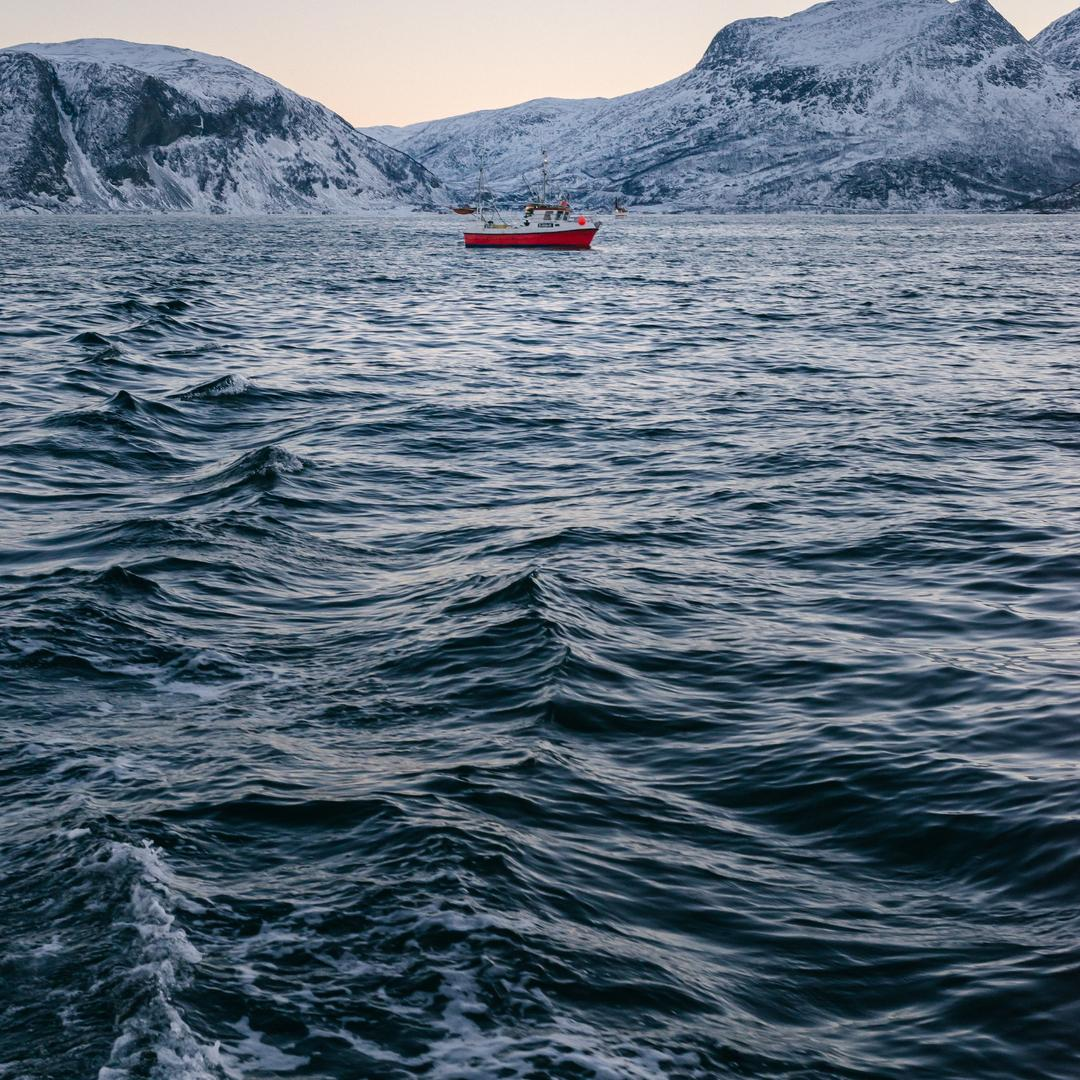
\includegraphics[width=\marginparwidth]{test1}
%   \caption{This is how the figure captions are displayed.}
% \end{marginfigure}

%   \subsubsection{Subsubsection Heading}
%   \lipsum[22]
%   \begin{nthm}
%     There are infinitely many primes. In particular,
%     \begin{equation}
%       \frac{1}{\zeta(s)} = \prod_{i} \left( 1 - \frac{1}{p^{s}_{i}} \right)
%     \end{equation}
%   \end{nthm}
%   \begin{proof}
%     The proof is trivial and left as an exercise. Deal with it!
%   \end{proof}

\section{Section Heading}
\lipsum[13]


Tables and figures have three options: in the usual text \texttt{figure} and \texttt{table} (with \texttt{tabularx}); or in the margin \texttt{marginfgure} and \texttt{margintable}; or as widetext with \texttt{widetext} or \texttt{figure*}, \texttt{table*}. Caption labels are also formatted as I wanted them to be.

\appendix
\section{Appendix Section Heading}
\lipsum[11]

\subsection{Appendix Subsection Heading}
\lipsum[12]

  \subsubsection{Appendix Subsubsection Heading}
  \lipsum[13]

\begin{center}
  \vspace*{1em}
  \rule{0.8\textwidth}{1pt}
\end{center}

\nocite{*}
{\small \bibliography{references}}

\end{document}